\chapter{Testy nowej metody}

W tym rozdziale zostaną przedstawione porównania opracowanej metody. \linebreak W pierwszej kolejności zaprezentowane zostanie zestawienie z metodą wytrenowaną z wykorzystaniem paradygmatu end-to-end, a zatem \textit{explicite} modelującą ocenę radiologa. Następnie przedstawione zostanie porównanie z wynikami prac algorytmu oceniającego proces gojenia się ścięgna Achillesa bazującego na danych z ultrasonografii. Ostatnie zestawienie dotyczy porównania wyników z oceną biomechaniczną.

Zarówno metoda oparta o paradygmat end-to-end jak i o dane ultrasonograficzne są wynikiem prac, w których autor tej rozprawy był współautorem, nadzorował grupę studentów opracowujących finalne rozwiązania oraz tworzył plan badań. \linebreak W przypadku oceny biomechanicznej prace nad metodą zrealizowane zostały w całości przez mgr Magdalenę Syrek z Carolina Medical Center w Warszawie, zatem wartością dodaną tej rozprawy jest przedstawione porównanie.   

\section{Porównanie z metodą opartą o paradygmat end-to-end}
\label{seq:end-to-end}
W tej sekcji podejście do oceny gojenia się ścięgna Achillesa realizowane przy pomocy opracowanej metody zostało porównana z podejściem bazującym na metodzie opartej o paradygmat end-to-end, modelującej \textit{explicite} ocenę radiologa. Do tego zadania zostały wykorzystane trzy architektury sieci konwolucyjnych opisane w Rozdziale \ref{CNNs} tj. AlexNet, GoogLeNet (Inception-v3) i ResNet z 50-cioma warstwami konwolucyjnymi (ResNet-50). Wszystkie trzy architektury zostały zmodyfikowane poprzez zastąpienie końcowej warstwy klasyfikacyjnej warstwą regresji z pojedynczym wyjściem \linebreak i funkcją kosztu zdefiniowaną jako średni błąd kwadratowy. W skutek tego podejścia algorytm szkolony jest w celu minimalizacji błędu pomiędzy predykcją sieci neuronowej, a wartościami parametrów z wzorca odniesienia. 

Dane wejściowe dla metody bazującej na end-to-end dobrano zgodnie z rutynowo stosowanymi technikami. A zatem do szkolenia się sieci wykorzystano powiększony zestaw treningowy, ograniczony do danych 44-ech pacjentów treningowych, zawierających sekwencje wybrane w toku eksperymentów przedstawionych w p. \ref{seq:protocol_selection}: T2 $^\ast$ GRE, T2 $^\ast$ GRE TE\_MIN i PD. Tym razem nie zdecydowano się na zawężenie zbioru danych tylko do jednej sekwencji RM, z uwagi na potrzebę maksymalizacji liczby próbek. Nie zdecydowano się również na pełny zbiór wszystkich sekwencji, z uwagi na różnice w danych, które mogłyby zaburzyć proces szkolenia się. 

Do szkolenia zastosowano metodę kroswalidacji z podziałem na 4 segmenty. Dla każdego z parametrów z wzorca odniesienia wyszkolono osobną sieć. Wyliczono miary MAE z informacją na temat błędu średniej, MAX-AE i Corr stosowane również w poprzednim rozdziale. Wyniki zestawiono w Tab. \ref{tab:end-to-endTrain}.
\vspace{10px}
\renewcommand{\arraystretch}{1.2}
\begin{table}[ht]
%\vspace{-px}
\scriptsize
\setlength{\tabcolsep}{1pt}
\centering
\caption{Wyniki szkolenia się sieci w paradygmacie end-to-end z wykorzystaniem zbioru treningowego. Pogrubieniem oznaczono najlepsze rezultaty.}
\label{tab:end-to-endTrain}
\begin{tabular}{lc||c|c|c|c|c|c}
	%\hline
	&& \textbf{SCT} & \textbf{TT} & \textbf{STE} & \textbf{TE} & \textbf{TU} & \textbf{TisE}\\ \hline \hline
	AlexNet$_{e}$ & MAE & 1,04$\pm$0,05 & 0,82$\pm$0,04 & 0,95$\pm$0,07 & 0,88$\pm$0,06 & 1,03$\pm$0,06 & 0,78$\pm$0,04  \\
	&MAX-AE & 1,91 & 1,67 & 2,39 & 2,20 & 1,90 & 1,35\\ 
	&Corr & 0,82 & \textbf{0,72} & \textbf{0,13} & 0,70 & 0,50 & 0,83 \\ \hline
	Inception-v3$_{e}$ & MAE & 0,88$\pm$0,05 & \textbf{0,75}$\pm$0,04 & \textbf{0,82}$\pm$0,05 & \textbf{0,78}$\pm$0,03 & \textbf{0,91}$\pm$0,05 & \textbf{0,67}$\pm$0,04 \\
	&MAX-AE & 1,57 & \textbf{1,44} & \textbf{1,93} & \textbf{1,17} & \textbf{1,85} & \textbf{1,11} \\ 
	&Corr & \textbf{0,85} & \textbf{0,72} & 0,05 & \textbf{0,72} & \textbf{0,52} & \textbf{0,84} \\ \hline
	ResNet-50$_{e}$ & MAE & \textbf{0,64}$\pm$0,03 & 0,98$\pm$0,04 & 0,83$\pm$0,06 & 0,89$\pm$0,03 & 1,06$\pm$0,06 & 1,10$\pm$0,05  \\
	&MAX-AE & \textbf{1,21} & 1,79 & 1,94 & 1,43 & 2,42 & 2,36\\
	&Corr & 0,06 & 0,21 & 0,00 & 0,11 & 0,14 & 0,11\\
	
	
\end{tabular}
%\vspace{-0.5cm}
\end{table}
\renewcommand{\arraystretch}{1}

Z uwagi na wyniki korelacji sieci ResNet-50$_{e}$, model ten został odrzucony z dalszej analizy. Niskie Corr jest prawdopodobnie efektem nadmiernego dopasowania. W skrajnym przypadku uśredniona korelacja równa jest 0,00 (parametr STE), co wynika z predykcji stałych wartości dla całego okresu gojenia się i błędów numerycznych związanych z tym faktem. 

W przypadku modeli AlexNet$_{e}$ i Inception-v3$_{e}$ nie ma istotnych statystycznie różnic dotyczących liczonych średnich. Sieć Inception-v3$_{e}$ charakteryzują natomiast mniejsze błędy maksymalne tj. MAX-AE. Na zbiorze testowym sprawdzono również, że nie ma efektu nadmiernego dopasowania modelu Inception-v3$_{e}$, co w podsumowaniu skutkowało wyborem tej architektury do dalszych porównań.

Model Inception-v3$_{e}$ zestawiono w Tab. \ref{tab:end-to-end_testset} z proponowaną przez autora tej pracy metodą meta-regresji opartą o algorytm SVR (SVR), porównując wyniki na zbiorze testowych 4-ech pacjentów.  
\vspace{10px}
\renewcommand{\arraystretch}{1.2}
\begin{table*}[h]
	\caption{Porównanie wyników wnioskowania z wykorzystaniem zbioru testowego dla metody proponowanej tj. SVR oraz metody wyszkolonej w paradygmacie end-to-end. Pogrubieniem oznaczono najlepsze rezultaty, a kolorem czerwonym istotne statystycznie różnice w liczonych średnich ($p$ $<$ 0,05).}
	\scriptsize
	\begin{center}
		\begin{tabular}{lc||c|c|c|c|c|c}
			\textbf{Model} & & \textbf{SCT} & \textbf{TT} & \textbf{STE} & \textbf{TE} & \textbf{TU} & \textbf{TisE}\\ \hline \hline
			Inception-v3$_{e}$ & MAE & 1,12$\pm{0,08}$ & 0,80$\pm{0,04}$ & 1,40$\pm{0,07}$ & \textbf{0,89}$\pm{0,05}$ & 1,08$\pm{0,04}$ & \textcolor{red}{\textbf{0,69}}$\pm{0,07}$ \\
			& MAX-AE & \textbf{2,14} & \textbf{1,01} & 2,13 & \textbf{1,18} & \textbf{1,44} & \textbf{0,78} \\
			& Corr & 0,82 & 0,77 & 0,05 & 0,59 & 0,52 & 0,77 \\ \hline
			SVR & MAE & \textbf{1,05}$\pm0,06$ & \textcolor{red}{\textbf{0,56}}$\pm0,03$ & \textcolor{red}{\textbf{0,75}}$\pm0,04$ & 0,91$\pm0,05$ & \textcolor{red}{\textbf{0,91}}$\pm0,04$ & $0,94\pm0,05$\\
			& MAX-AE & 2,62 & 1,82 & \textbf{1,92} & 2,54 & 2,01 & 2,38 \\
			& Corr & \textbf{0,85} & \textbf{0,85} & \textcolor{red}{\textbf{0,31}} & \textcolor{red}{\textbf{0,72}} & \textcolor{red}{\textbf{0,65}} & \textbf{0,80} 
		\end{tabular}
	\end{center}
	\label{tab:end-to-end_testset}
\end{table*}
\renewcommand{\arraystretch}{1}

Metoda SVR osiąga istotne statystycznie wyższe wartości Corr dla parametrów STE, TE i TU i MAE dla parametrów TT, STE i TU. Natomiast tylko w jednym z parametrów (tj. STE) charakteryzuje się niższym błędem MAX-AE. 

Dobre wyniki MAX-AE modelu Inception-v3$_{e}$ są skutkiem sposobu treningu polegającego na \textit{explicite} modelowaniu wzorca odniesienia, co przekłada się na zadanie minimalizowania maksymalnych błędów. Trudność w interpretacji polega na fakcie, że maksymalne błędy mogą być wynikiem błędu algorytmu, jak również pojedynczymi omyłkami doświadczonego radiologa, który z uwagi np. na zmęczenie bądź inne dystrakcje percepcji popełnił błąd w ocenie.

Jeden istotnie lepszy wynik sieci Inception-v3$_e$ w MAE dla TisE jest intuicyjny. Jest to jedyny parametr oceniany na zewnątrz ścięgna, gdzie fuzja cech nie powinna mieć bezpośredniego wpływu na polepszenie rezultatu. 

Wyniki Corr świadczą, że cechy wykorzystywane w metodzie SVR do oceny procesu gojenia się pozwalają na ocenę trendu z lepszą dokładnością niż metoda oparta o paradygmat end-to-end. W podsumowaniu należy jednak również podkreślić zasadnicze praktyczne różnice między oboma podejściami. Do rozwoju metody end-to-end niezbędna jest pełna informacja od radiologa tj. ocena 6-ciu parametrów w kolejnych krokach czasowych. Średnio jest to około jedna godzina pracy na pacjenta. Proponowana przez autora metoda w części wykorzystuje sieć wyszkoloną na bazie etykiet wyższego poziomu tj. rozróżniających jedynie oznaczenia zdrowych i chorych tkanek. Takie szkolenie jest nazywane \textit{słabo-nadzorowanym} (w odróżnieniu od w \textit{pełni-nadzorowanego}, w paradygmacie end-to-end). Dalszy rozwój proponowanej metody można zatem uzyskać przy wykorzystaniu danych oznaczonych jako chory lub zdrowy (ulepszanie ekstraktora cech) oraz znacząco mniejszego zbioru pacjentów z segmentacją ścięgna, który służyłby do sporadycznych ulepszeń etapu meta-regresji. 

Minusem podejścia meta-regresji jest natomiast wymóg informacji o ROI. W kontekście badań na danych z projektu START problem oznaczenia nie istniał, gdyż obszar ścięgna był rutynowo etykietowany do celów innych badań. W przypadku bardziej generycznym, gdzie nie istniałyby oznaczenia obszaru ścięgna, zaistniałaby konieczność dodatkowej pracy radiologa w wymiarze około 10 minut na pacjenta (przy założeniu wykorzystania odpowiedniego oprogramowanie np. Osirix \cite{Rosset2004} lub VisNow \cite{Nowinski_Borucki_2014}). Nowoczesne metody pokazują możliwość zautomatyzowania tego procesu. Dla przykładu, wstępne prace dr. Jędrzeja Nowosielskiego i dr. Piotra Regulskiego oraz autora tej pracy pokazują, że skuteczne w tym zakresie mogą być sieci typu \textit{fully convolutional neural networks}. Przykład działania takiej architektury, a dokładniej U-Net zaproponowanej w \cite{Ronneberger2015}, można zaobserwować na Rys. \ref{fig:segmentacja}. 

\begin{figure}[h]
	\centering
	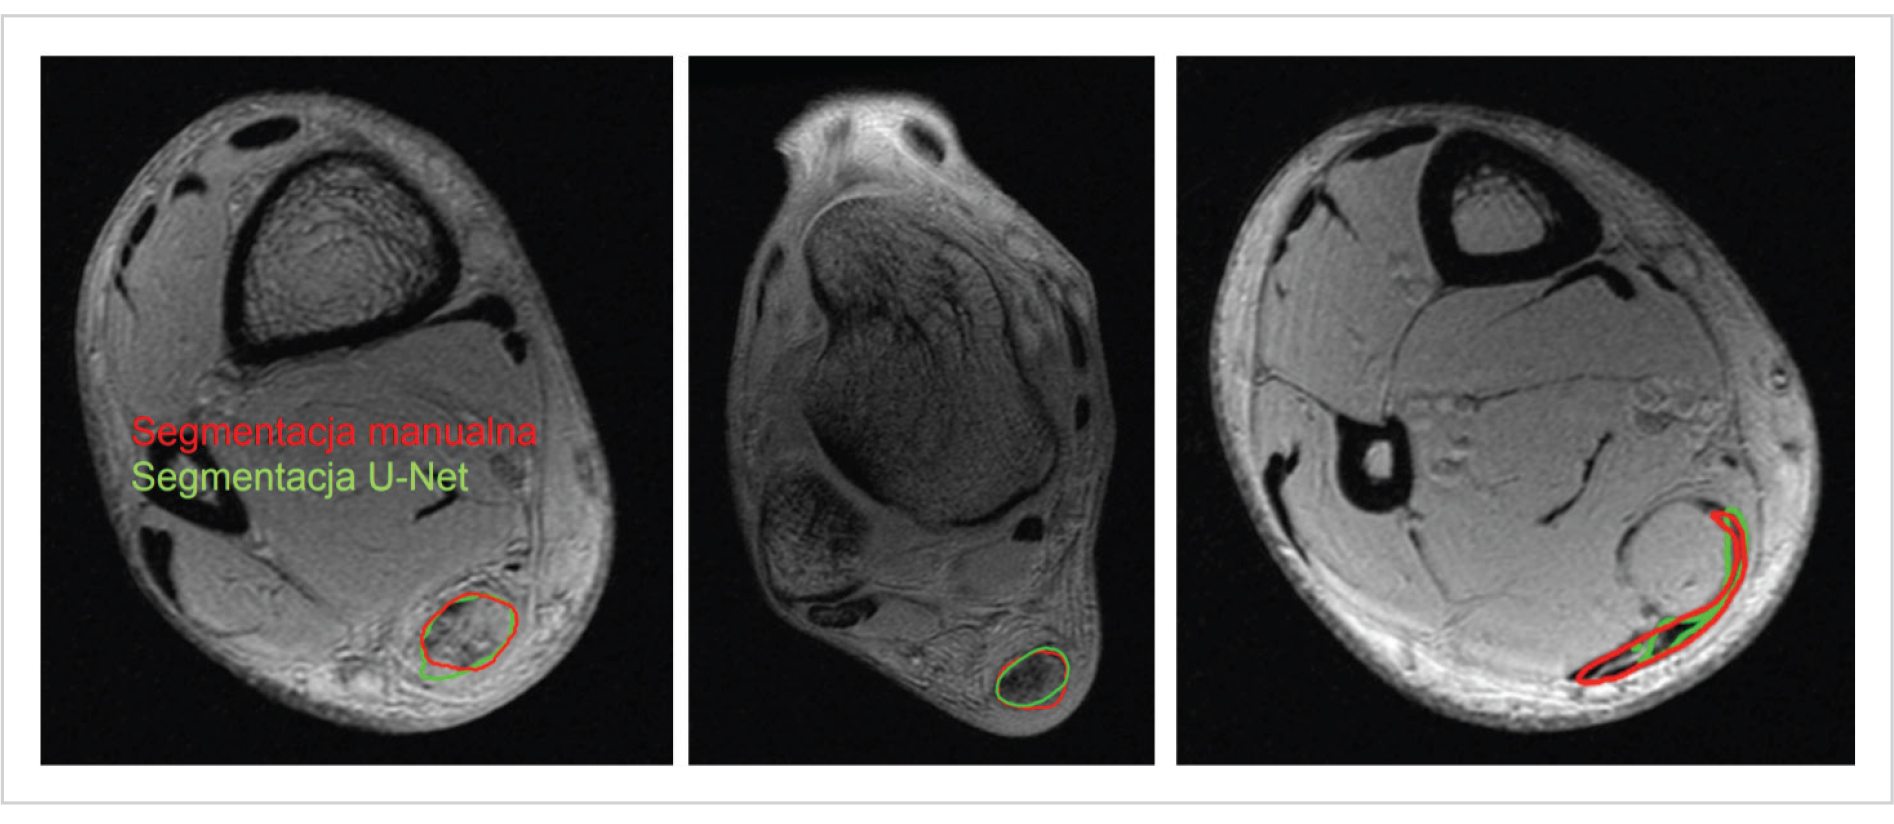
\includegraphics[width=1\textwidth]{figures/Segmentacja.jpg}
	\caption{Automatyczna segmantacja ROI z wykorzystaniem głębokich sieci neuronowych.}\label{fig:segmentacja}
\end{figure}

Kolorem czerwonym oznaczono obszar segmentacji manualnej wykonanej przez eksperta radiologa. Kolorem zielonym efekt segmentacji automatycznej. Miara DICE (zob. \cite{Zou2004}) dla otrzymanych obrazów wynosi około 0,75 i świadczy o wysokiej jakości segmentacji oraz o obiecującym kierunku tego rodzaju prac. Z uwagi jednak na fakt, że jest to obszerny, kolejny wątek dotyczący ścięgna Achillesa widocznego w obrazowaniu medycznym, wymagający znacznego poszerzenia omawianej problematyki, nie został on dalej rozwinięty w tej pracy.

Ciekawym elementem rozwoju automatycznej oceny byłaby również fuzja obu metod tj. podmiana ekstraktora cech DL trenowanego na binarnie oznaczonym zbiorze na ekstraktor uzyskany w modelu Inception-v3$_e$. Jednak z uwagi na omawiane problemy praktyczne z dalszym rozwojem tak utworzonej metody oraz brak obiecujących rezultatów w przeprowadzonych przez autora tej pracy badaniach wstępnych, taka propozycja nie została uwzględniona w prezentowanej rozprawie. 

\section{Porównanie z metodą opartą o dane z USG}
\label{seq:comp-usg}
W tej sekcji opracowana metoda została porównana z automatyczną oceną bazującą na danych z Ultrasonografii. Ponownie, do utworzenia metody opartej o USG, wykorzystano konwolucyjne sieci neuronowe, a dokładniej AlexNet, Inception-v3 \linebreak i ResNet-50 oraz wykorzystano omówiony w poprzedniej sekcji paradygmat~end-to-end. 

Dane dla metody opartej o Ultrasonografię pochodziły od tych samych pacjentów z projektu START, co w przypadku badań RM. Stosowano się również do identycznych odstępów czasowych. Z przyczyn praktycznych zmniejszyła się jedynie grupa odniesienia, która w tym przypadku wyniosła 18-stu zdrowych ochotników. Badania zrealizowano z wykorzystaniem aparatu GE 3D high-resolution Voluson E8 Expert z liniową sondą (5--18 MHz). Jako dane wejściowe wykorzystano informacje z trybu B (zob. p. \ref{USG}), których ostateczna liczba wyniosła 565 skanów 3D. 

Dane USG są zbliżone do izotropowych dlatego utworzono zbiory zarówno \linebreak w oparciu o przekroje w płaszczyźnie poprzecznej jak i strzałkowej (wykorzystując obrazy, gdzie widoczne jest ścięgno):
\begin{itemize}[noitemsep,nolistsep]
	\item zbiór treningowy USG (strzałkowy) -- zawierał 253.639 2D przekrojów w płaszczyźnie strzałkowej, w tym 245.366 pochodzących od chorych 44-ech pacjentów oznaczonych przez radiologa i 8.273 pochodzących od zdrowych ochotników.
	\item zbiór treningowy USG (poprzeczny) -- zawierał 467.548 2D przekrojów w płaszczyźnie poprzecznej, w tym 450.816 pochodzących od chorych 44-ech pacjentów oznaczonych przez radiologa i 16.732 pochodzących od zdrowych ochotników. 
\end{itemize}

Wizualizacja przykładowych danych USG znajduje się na Rys. \ref{fig:US_sample}.
\begin{figure}[h!]
	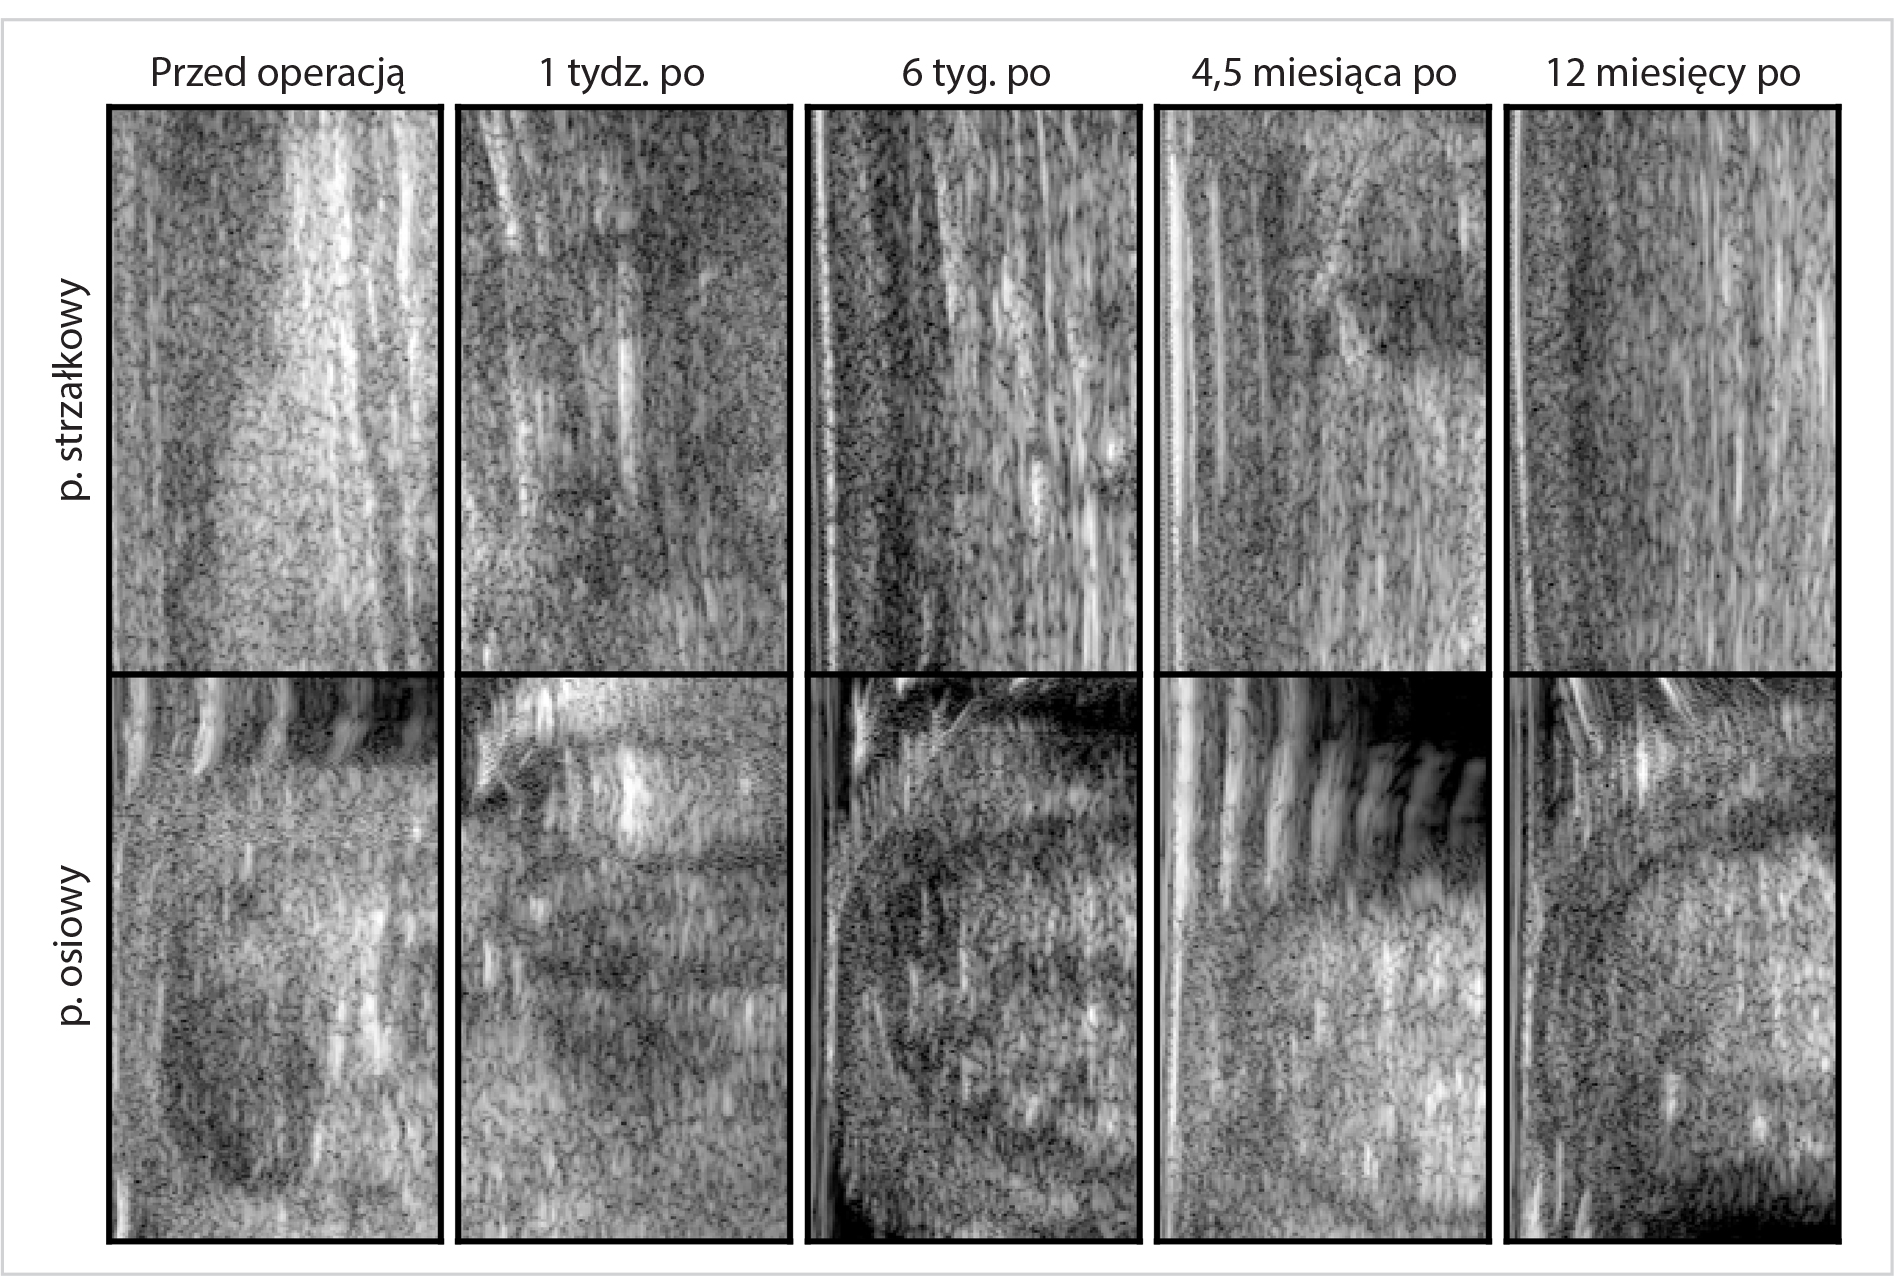
\includegraphics[width=\textwidth]{figures/Data_US_sample.jpg}
	\caption{Wizualizacja przykładowych danych USG w przekrojach poprzecznych i strzałkowych, w kolejnych tygodniach po zszyciu ścięgna.}
	\label{fig:US_sample}
\end{figure}
W ogólności można zaobserwować ułożenie włókien ścięgnistych na przekrojach strzałkowych \linebreak i teksturę oraz tkanki otaczające ścięgno na przekrojach poprzecznych. Jednak szczegółowa analiza załączonych obrazów może być wykonana jedynie przez specjalistę radiologa. 

Utrudniona w stosunku do obrazów RM interpretacja ma związek z obecnymi artefaktami w USG i z szumem ziarnistym tworzącym losowe wzorce. Jakość obrazu obniża również jego wartość kliniczną, co wskazują analizy zamieszczone w tej pracy jak i w wielu pracach innych autorów (zob. np. \cite{Khan2003, Ibrahim2013}). Dlatego na początku zdecydowano się przeprowadzić test polegający na prostym zadaniu klasyfikacji binarnej chory/zdrowy (podobnie jak dla badań RM zamieszczonych w p. \ref{binaryMRI}). Miało \linebreak to na celu porównanie możliwości interpretacji wnioskowania na podstawie obrazów RM i USG. Wyniki dla szkolenia z wykorzystaniem kroswalidacji z 4-ema segmentami zamieszczono w Tabeli \ref{tab:usg-binary}.
\renewcommand{\arraystretch}{1.2}
\begin{table}[]
	\centering
	\scriptsize
	\setlength{\tabcolsep}{3pt}
	\setlength\extrarowheight{2pt}
	\caption{Wyniki szkolenia się sieci dla problemu binarnego na zbiorze treningowym dla danych z USG. Pogrubieniem oznaczono najlepsze wyniki ACC.}
	\label{tab:usg-binary}
	\begin{tabular}{l||c|c|c||c|c|c}
		%\hline
		& \multicolumn{3}{c}{\textbf{p. strzałkowy}} & \multicolumn{3}{c}{\textbf{p. poprzeczny}} \\
		\textbf{Model} & \textbf{ACC} & \textbf{PPV} & \textbf{TPR} & \textbf{ACC} & \textbf{PPV} & \textbf{TPR} \\ \hline \hline
		AlexNet$_{bu}$ & 0,85$\pm$0,09 & 0,92$\pm$0,08 & 0,78$\pm$0,11 & 0,843$\pm$0,07 & 0,93$\pm$0,06 & 0,73$\pm$0,11  \\ \hline
		Inception-v3$_{bu}$ & \textbf{0,92}$\pm$0,05 & 0,97$\pm$0,04 & 0,90$\pm$0,06 & 0,90$\pm$0,05 & 0,95$\pm$0,03 & 0,87$\pm$0,07 \\ \hline
		ResNet-50$_{bu}$ & 0,91$\pm$0,04 & 0,96$\pm$0,05 & 0,89$\pm$0,08 & \textbf{0,91}$\pm$0,05 & 0,95$\pm$0,04 & 0,88$\pm$0,06 \\ 
	\end{tabular}
\end{table}
\renewcommand{\arraystretch}{1}

Wszystkie modele wytrenowano oddzielnie na przekrojach poprzecznych i oddzielnie na strzałkowych. Żeby zbalansować dane, przekroje od zdrowych ochotników powiększono poprzez odbicie, a przekroje od chorych pacjentów próbkowano. Dokładność dla najlepszego modelu w przekroju poprzecznym wyniosła 91,6\%, a w przekroju strzałkowym 91,2\%. Dla porównania, dokładność binarnej klasyfikacji na danych z RM wyniosła 99,83\%. Wyniki te potwierdzają możliwość lepszej interpretacji danych RM dla zadanego problemu, jednak nie dyskryminują USG. W celu polepszenia rezultatów eksperymentowano również z możliwością klasyfikacji binarnej z wykorzystaniem jedynie obszaru ROI, jednak działania te przyniosły odwrotny~skutek.  
\vspace{6px}
\renewcommand{\arraystretch}{1.2}
\begin{table}[h]
	\scriptsize
	\setlength{\tabcolsep}{3pt}
	\centering
	\caption{Wyniki szkolenia sieci dla danych z USG. Pogrubieniem oznaczono najlepsze rezultaty, osobno dla przekrojów poprzecznych i strzałkowych}
	\label{tab:usg_train_cross-validation}
	\begin{tabular}{lc||c|c|c|c|c|c}
		%\hline
		& & \multicolumn{6}{c}{\textbf{p. strzałkowy}} \\
		\textbf{Model} & & \textbf{SCT} & \textbf{TT} & \textbf{STE} & \textbf{TE} & \textbf{TU} & \textbf{TisE} \\ \hline \hline
		AlexNet$_{eus}$ & MAE & 0,96$\pm$0,20 & 0,80$\pm$0,13 & 0,82$\pm$0,14 & 0,95$\pm$0,20 & 0,87$\pm$0,20 & 1,08$\pm$0,23  \\
		& MAX-AE & 1,75 & 1,32 & 1,87 & 1,35 & 1,61 & 2,03 \\ 
		& Corr & 0,53 & 0,69 & 0,11 & \textbf{0,68} & 0,31 & 0,22 \\ \hline
		Inception-v3$_{eus}$ & MAE & \textbf{0,88}$\pm$0,16 & \textbf{0,67}$\pm$0,11 & \textbf{0,80}$\pm$0,15 & 0,82$\pm$0,11 & \textbf{0,84}$\pm$0,11 & \textbf{0,93}$\pm$0,15  \\
		& MAX-AE & 1,69 & 1,32 & 1,69 & \textbf{1,31} & \textbf{1,58} & \textbf{1,64} \\ 
		& Corr & \textbf{0,83} & \textbf{0,71} & 0,19 & 0,64 & \textbf{0,56} & \textbf{0,71} \\ \hline
		ResNet-50$_{eus}$ & MAE & 0,89$\pm$0,06 & 0,74$\pm$0,07 & 0,83$\pm$0,11 & \textbf{0,81}$\pm$0,15 & 0,92$\pm$0,15 & 0,99$\pm$0,15 \\
		& MAX-AE & \textbf{1,53} & \textbf{1,22} & \textbf{1,64} & 1,43 & 1,67 & 1,71 \\
		& Corr & 0,62 & 0,38 & \textbf{0,23} & 0,62 & 0,12 & 0,43 \\ \hline \hline
		& & \multicolumn{6}{c}{\textbf{p. poprzeczny}} \\
		
		AlexNet$_{euo}$ & MAE & \textbf{0,98}$\pm$0,20 & 0,83$\pm$0,16 & 0,82$\pm$0,17 & 0,94$\pm$0,26 & 0,95$\pm$0,25 & 0,86$\pm$0,14  \\
		& MAX-AE & \textbf{1,79} & \textbf{1,36} & 1,86 & 1,41 & 1,61 & 1,59 \\ 
		& Corr & 0,45 & 0,62 & 0,20 & 0,60 & 0,03 & 0,59 \\ \hline
		Inception-v3$_{euo}$ & MAE & 1,03$\pm$0,23 & \textbf{0,70}$\pm$0,12 & \textbf{0,76}$\pm$0,13 & \textbf{0,86}$\pm$0,09 & 0,87$\pm$0,16 & \textbf{0,85}$\pm$0,12  \\
		& MAX-AE & 2,52 & \textbf{1,45} & \textbf{1,45} & \textbf{1,24} & 1,67 & \textbf{1,56} \\ 
		& Corr & \textbf{0,77} & \textbf{0,69} & \textbf{0,22} & \textbf{0,65} & \textbf{0,55} & \textbf{0,72} \\ \hline
		ResNet-50$_{euo}$ & MAE & 1,05$\pm$0,15 & 0,78$\pm$0,16 & 0,80$\pm$0,12 & 1,02$\pm$0,12 & \textbf{0,87}$\pm$0,12 & 0,91$\pm$0,14 \\
		& MAX-AE & 1,98 & 1,51 & 1,59 & 1,63 & \textbf{1,45} & 1,57 \\
		& Corr & 0,52 & 0,47 & 0,21 & 0,64 & 0,18 & 0,57 \\ 
		
	\end{tabular}
\end{table}
\renewcommand{\arraystretch}{1}

Kolejnym krokiem eksperymentu było porównanie jakości oceny procesu gojenia. W badaniu wykorzystano ponownie paradygmat end-to-end i zmianę warstwy klasyfikującej na regresję z funkcją kosztu określoną jako średni błąd kwadratowy. Dla tej metody próbowano również odtworzyć schemat sprawdzony dla RM, bazujący na treningu binarnym oraz ekstrakcji i redukcji cech. W przypadku USG otrzymane wyniki nie były jednak na tyle satysfakcjonujące, aby zamieszczać je w tej pracy. Ostatecznie, wyniki szkolenia sieci w paradygmacie end-to-end zamieszczono w Tabeli \ref{tab:usg_train_cross-validation}.

Między modelami nie uzyskano statystycznie istotnych różnic  dla liczonych średnich. Ostatecznie na bazie liczby najmniejszych błędów MAX-AE, odpowiednio 7 dla Inception-v3 i 4 dla ResNet-50 dokonano wyboru tych dwóch modeli do porównań z metodą bazującą na meta-regresji. W tym celu wyniki MAE, MAX-AE i Corr zostały wyliczone dla zbioru pacjentów testowych i zebrane w Tabeli \ref{tab:USGvsRM-cross-validation}.
\vspace{6px}
\renewcommand{\arraystretch}{1.2}
\begin{table}[h]
	\scriptsize
	\setlength{\tabcolsep}{1pt}
	\centering
	\caption{Porównanie wyników oceny automatycznej, bazującej na danych USG i RM, dla pacjentów ze zbioru testowego. Pogrubieniem oznaczono najlepsze wyniki. Kolorem czerwonym oznaczono poprawę w stosunku do kolejnego wyniku istotną statystycznie z $p$ $<$ 0,05.}
	\label{tab:USGvsRM-cross-validation}
	\vspace{-0.5cm}
	\begin{tabular}{lc||c|c|c|c|c|c}
		%\hline
		& & \multicolumn{6}{c}{\textbf{USG -- p. strzałkowy}} \\
		\textbf{Model} & & \textbf{SCT} & \textbf{TT} & \textbf{STE} & \textbf{TE} & \textbf{TU} & \textbf{TisE} \\ \hline \hline
		Inception-v3$_{eus}$ & MAE & \textbf{0,81}$\pm$0,19 & 0,63$\pm$0,03 & \textbf{0,56}$\pm$0,09 & 0,85$\pm$0,10 & 0,54$\pm$0,02 & 0,87$\pm$0,14 \\
		& MAX-AE & 1,59 & 1,79 & 1,7 & \textbf{1,25} & \textbf{1,38} & 1,69 \\
		& Corr & 0,80 & 0,77 & 0,31 & 0,52 & \textbf{0,69} & 0,62 \\ \hline
		ResNet-50$_{eus}$ & MAE & 0,88$\pm$0,16 & 0,65$\pm$0,07 & 0,66$\pm$0,04 & 0,83$\pm$0,12 & 0,75$\pm$0,06 & 0,93$\pm$0,11 \\
		& MAX-AE & \textbf{1,49} & \textbf{1,26} & 1,74 & 1,48 & 1,78 & 1,71 \\
		& Corr & 0,60 & 0,55 & 0,25 & 0,55 & 0,34 & 0,56 \\
		\hline \hline
		& & \multicolumn{6}{c}{\textbf{USG -- p. poprzeczny}} \\
		
		Inception-v3$_{euo}$ & MAE & 0,84$\pm$0,27 & 0,75$\pm$0,7 & 0,58$\pm$0,05 & 0,83$\pm$0,05 & \textcolor{red}{\textbf{0,53}}$\pm$0,08 & \textbf{0,83}$\pm$0,15 \\
		& MAX-AE & 2,8 & 1,46 & \textbf{1,51} & 1,27 & 1,63 & 1,65 \\
		& Corr & 0,69 & 0,68 & \textbf{0,45} & 0,51 & 0,66 & 0,68 \\ \hline
		ResNet-50$_{euo}$ & MAE & 0,92$\pm$0,18 & 0,76$\pm$0,16 & 0,68$\pm$0,04 & \textbf{0,81}$\pm$0,08 & 0,65$\pm$0,10 & 0,94$\pm$0,05 \\
		& MAX-AE & 2,01 & 1,56 & 1,61 & 1,69& 1,43 & \textbf{1,58}\\
		& Corr & 0,55 & 0,57 & 0,35 & 0,44 & 0,39 & 0,61 \\ \hline \hline
		& & \multicolumn{6}{c}{\textbf{Rezonans magnetyczny}} \\
		
		SVR & MAE & $1,05\pm0,06$ & \textbf{0,56}$\pm0,03$ & $0,75\pm0,04$ & $0,91\pm0,05$ & $0,91\pm0,04$ & $0,94\pm0,05$\\
		& MAX-AE & 2,62 & 1,82 & 1,92 & 2,54 & 2,01 & 2,38 \\
		& Corr   & \textbf{0,85} & \textbf{0,85} & 0,31 & \textcolor{red}{\textbf{0,72}} & 0,65 & \textcolor{red}{\textbf{0,80}} \\
		 
	\end{tabular}
\end{table}
\renewcommand{\arraystretch}{1}

Podobnie jak w przypadku porównania z modelami trenowanymi na danych RM w paradygmacie end-to-end, maksymalne błędy MAX-AE uzyskane przez modele wytrenowane na danych USG były w każdym przypadku mniejsze niż w przypadku metody opartej na fuzji. Ponownie jest to efekt sposobu szkolenia bazującego \textit{explicite} na ocenach radiologa. Bardzo interesujący jest wynik istotnej statystycznie poprawy w parametrze TU realizowanej przez model Inception-v3. Oceniana jest tam jednorodność ścięgna, dobrze widoczna w USG w przekrojach strzałkowych (wynik MAE równy 0,54) jak i przekrojach poprzecznych (MAE równe 0,53). Metoda fuzji uzyskała natomiast statystycznie istotną poprawę w przypadku Corr dla parametrów związanych z obrzękami (TisE, TE), gdzie dominują efekty związane z ukrwieniem tkanek podczas procesu gojenia się.

Bazując na powyższych rezultatach można wnioskować, że metoda oparta o dane USG może być komplementarna z proponowaną oceną bazującą na danych \linebreak z RM, zwłaszcza w kontekście oceny parametru TU. Do tego celu potrzebna jest dokładna analiza i zrozumienie podstaw wnioskowania sieci opartej o USG, a następnie wybór oraz realizacja odpowiedniej metody fuzji.

\section{Porównanie z metodą opartą o badania biomechaniczne}
\label{seq:comp-biomechanics}
W tej sekcji opracowana metoda została porównana z wynikami badań biomechanicznych i wynikami funkcjonalnego testu ATRS. Badania te były realizowane w ramach protokołu monitorowania rehabilitacji pacjentów opracowanego w klinice Carolina Medical Center (zob. p. \ref{biomechanika}). 

W ramach projektu START możliwe było zebranie danych dla 30-tu spośród 60-ciu pacjentów. Dane zawierały wyniki pomiaru zrealizowanego w dwóch krokach czasowych tj. w 26-tym i 52-rugim tygodniu po operacji. Po wstępnych analizach, do porównań w tej pracy wykorzystano zebrane wyniki ATRS i deficyty sił mięśniowych będące rezultatem badań biomechanicznych. Dokładniej, określono 16-cie takich deficytów oznaczonych dalej w tej pracy \textit{d1}--\textit{d16}\index{\textit{d1}--\textit{d16} -- kolejne deficyty biomechaniczne}. W czterech pozycjach tj. kolano zgięte i wyprostowane oraz staw skokowy zgięty wyprostowany zrealizowano pomiary w warunkach izometrii i izokinetyki dla trzech prędkości kątowych 60$^\circ$/s, 120$^\circ$/s oraz 180$^\circ$/s  

Z uwagi na dużą liczbę pomiarów, zdecydowano się w pierwszej kolejność \linebreak na przeprowadzenie analizy czynników głównych i identyfikację nowych zmiennych wyjaśniających w największym stopniu wariancję w zebranym zbiorze danych. Wyniki podsumowano w Tabeli \ref{tab:pca-muscles}.

\begin{table}[h]
	\centering
	\setlength{\tabcolsep}{3pt}
	\setlength\extrarowheight{2pt}
	\caption{Wyniki analizy czynników głównych dla 16-tu pomiarów deficytów mięśniowych w warunkach izometrii i izokinetyki. Oznaczono ładunki, gdzie wartość modułu jest większa niż 0,7.}
	\label{tab:pca-muscles}
	\begin{tabular}{c|c|c|c|c}
		%\hline

		Zmienna&Czynnik1&Czynnik2&Czynnik3&Czynnik4 \\
		\hline \hline
		\textit{d1}&\textbf{-0,77}&0,16&-0,04&-0,25 \\
		\hline
		\textit{d2}&0,32&\textbf{-0,74}&0,038&-0,044 \\
		\hline
		\textit{d3}&\textbf{-0,81}&0,26&-0,17&-0,24 \\
		\hline
		\textit{d4}&0,09&-0,62&-0,50&-0,38 \\
		\hline
		\textit{d5}&\textbf{-0,82}&0,13&-0,03&0,21 \\
		\hline
		\textit{d6}&0,31&-0,53&-0,53&0,42 \\
		\hline
		\textit{d7}&-0,67&-0,20&-0,34&-0,11 \\
		\hline
		\textit{d8}&-0,12&-0,34&-0,67&0,43 \\
		\hline
		\textit{d9}&-0,61&-0,01&-0,28&-0,36 \\
		\hline
		\textit{d10}&0,07&\textbf{-0,84}&0,26&0,02 \\
		\hline
		\textit{d11}&\textbf{-0,81}&-0,14&0,01&0,08 \\
		\hline
		\textit{d12}&-0,11&\textbf{-0,93}&-0,01&-0,01 \\
		\hline
		\textit{d13}&\textbf{-0,72}&-0,24&0,28&0,36 \\
		\hline
		\textit{d14}&-0,12&\textbf{-0,81}&0,33&-0,25 \\
		\hline
		\textit{d15}&-0,58&-0,32&0,39&0,53 \\
		\hline
		\textit{d16}&-0,17&-0,62&0,23&-0,36 \\
		\hline\hline
		Udział&0,28&0,27&0,10&0,09 \\

	\end{tabular}
\end{table}

Z czterech czynników dwa mają wyraźnie większy udział w wyjaśnianej wariancji, osiągając odpowiednio poziomy 28 i 27\%. Istotne jest również, że trzy z pięciu znaczących ładunków czynnikowych (\textit{d1}, \textit{d3}, \textit{d5}) dla pierwszego czynnika znajdują się w przedziale \textit{d1}--\textit{d8}, które skojarzone są z pozycją kolana prostego oraz, \linebreak że dla drugiego czynnika głównego sytuacja jest odwrotna i trzy z czterech ładunków czynnikowych (\textit{d10}, \textit{d12}, \textit{d14}) znajdują się w przedziale \textit{d9}--\textit{d16}, czyli badania przy kolanie zgiętym. 

Co oczywiste, pozycja kolana wpływa znacząco na wynik badania biomechanicznego, dlatego w ramach dalszej pracy zdecydowano się na  analizę czynnikową dla wyprostowanego i zgiętego kolana oddzielnie. Wyniki zostały przedstawione \linebreak w Tabeli \ref{tab:pca-muscles-knee-strait-bended}. 

Ponownie można zaobserwować charakterystyczne rozróżnienie. Pierwszy czynnik główny dla badania w pozycji kolana wyprostowanego zawiera ładunki znaczące o nieparzystych numerach, a drugi czynnik posiada znaczące ładunki o parzystych numerach. W przypadku badania w pozycji kolana zgiętego sytuacja jest odwrotna i analogicznie można zaobserwować rozróżnienie. W tym przypadku podział wynika z pozycji stawu skokowego. Ładunki o nieparzystych numerach posiadają czynniki związane z badaniami w zgięciu stawu skokowego, a o parzystych w wyproście. \linebreak Z uwagi na ten fakt do kolejnych porównań zostały zdefiniowane następujące 4 zmienne:
\begin{enumerate}[noitemsep,nolistsep]
	\item $ZZ$ -- wyniki dla pozycji kolano zgięte i staw skokowy zgięty.\index{$ZZ$ -- zmienna określająca deficyty biomechaniczne dla pozycji kolano zgięte i staw skokowy zgięty}
	\item $ZW$ -- wyniki dla pozycji kolano zgięte i staw skokowy wyprostowany.\index{$ZW$ -- zmienna określająca deficyty biomechaniczne dla pozycji kolano zgięte i staw skokowy wyprostowany}
	\item $WZ$ -- wyniki dla pozycji kolano wyprostowane i staw skokowy zgięty.\index{$WZ$ -- zmienna określająca deficyty biomechaniczne dla pozycji kolano wyprostowane i staw skokowy zgięty}
	\item $WW$ -- wyniki dla pozycji kolano wyprostowane i staw skokowy wyprostowany.\index{$WW$ -- zmienna określająca deficyty biomechaniczne dla pozycji kolano wyprostowane i staw skokowy wyprostowany}
\end{enumerate} 
\begin{table}[h!]
	\centering
	\setlength{\tabcolsep}{3pt}
	\setlength\extrarowheight{2pt}
	\caption{Wyniki analizy czynników głównych dla 16-tu pomiarów deficytów mięśniowych, oddzielnie dla pozycji kolana zgiętego i wyprostowanego. Oznaczono ładunki, gdzie wartość modułu jest większa niż 0,7.}
	\label{tab:pca-muscles-knee-strait-bended}
	\begin{tabular}{c|c|c||c|c|c}
		%\hline
		
		Zmienna&Czynnik1&Czynnik2&Zmienna&Czynnik1&Czynnik2 \\
		\hline \hline
		\textit{d1}&\textbf{-0,82}&-0,14&d9&-0,26&0,64 \\
		\hline
		\textit{d2}&-0,60&-0,37&d10&\textbf{-0,72}&-0,47 \\
		\hline
		\textit{d3}&\textbf{0,88}&-0,20&d11&-0,52&\textbf{0,73} \\
		\hline
		\textit{d4}&-0,36&-0,65&d12&\textbf{-0,83}&-0,34 \\
		\hline
		\textit{d5}&\textbf{0,83}&-0,26&d13&-0,65&0,64 \\
		\hline
		\textit{d6}&-0,57&-0,64&d14&\textbf{-0,81}&-0,43 \\
		\hline
		\textit{d7}&0,55&-0,60&d15&-0,67&0,40 \\
		\hline
		\textit{d8}&-0,03&\textbf{-0,80}&d16&-0,65&-0,38 \\
		\hline\hline
		Udział&0,41&0,26&&0,44&0,27 \\
		
	\end{tabular}
\end{table}

Każda z nowo powstałych zmiennych jest pierwszym czynnikiem analizy PCA dokonanej na czterech pomiarach: jednego dla izometrii i trzech dla izokinetyki. Takie podejście, w kontrze do zwykłej średniej arytmetycznej zapewnia ważenie wpływu poszczególnych składowych, co jest zgodne z naturą procesu, na który mierzone elementy mają różny wpływ. Dokładne zestawienie wyników dla nowych zmiennych znajduje się w Tabeli \ref{tab:bio-new-factors}.
\vspace{20px}
\begin{table}[h!]
	\centering
	\setlength{\tabcolsep}{3pt}
	\setlength\extrarowheight{2pt}
	\caption{Komponenty i ich udział, wchodzące w skład nowych zmiennych opisujących biomechanikę.}
	\label{tab:bio-new-factors}
	\begin{tabular}{c|c|c|c|c||c}
		Nowa zmienna&Zmienna1&Zmienna2&Zmienna3&Zmienna4&Udział (Czynnik1) \\
		\hline \hline
		$ZZ$&\textit{d9} (-0,61)&\textit{d11} (-0,88)&\textit{d13} (-0,92)&\textit{d15} (-0,77)&0,65\\
		\hline
		$ZW$&\textit{d10} (-0,86)&\textit{d12} (-0,91)&\textit{d14} (-0,92)&\textit{d16} (-0,77)&0,75\\
		\hline
		$WZ$&\textit{d1} (-0,85)&\textit{d3} (-0,90)&\textit{d5} (-0,87)&\textit{d7} (-0,72)&0,70\\
		\hline
		$WW$&\textit{d2} (-0,64)&\textit{d4} (-0,76)&\textit{d6} (-0,88)&\textit{d8} (-0,66)&0,55\\
		
		
	\end{tabular}
\end{table}

Otrzymany podział jest intuicyjny, niemniej jednak fakt otrzymania powyższych wyników w analizie numerycznej jest wartością dodaną potwierdzającą spójność danych i jakość przeprowadzonych badań przez fizjoterapeutów z Carolina Medical Center.  

W kolejnej tabeli (tj. Tabeli \ref{tab:bioVSatrs}) przedstawiono wyniki korelacji nowych zmiennych opisujących biomechanikę z wynikami testu ATRS. Badania ograniczono do tej podgrupy zestawu pomiarów przedstawionego w p. \ref{biomechanika}, gdyż wstępne analizy pokazały, ze grupa ta jest najbardziej homogeniczna biorąc pod uwagę wpływ ścięgna na pomiar. Inne badania zależą od zbyt wielu czynników czego implikacją w badanej grupie było brak powtarzalnych wzorców wynikających z deficytów samego ścięgna.
\vspace{10px}
\begin{table}[h]
	\centering
	\setlength{\tabcolsep}{3pt}
	\setlength\extrarowheight{2pt}
	\caption{Korelacja badań biomechanicznych z testem ATRS. Oznaczone wsp. korelacji są istotne z $p$ $<$ 0,05 dla $N$=30.}
	\label{tab:bioVSatrs}
	\begin{tabular}{c|c|c|c|c|c}
		&WW&WZ&ZW&ZZ&ATRS \\
		\hline \hline
		WW&1,0000&-0,2037&\textbf{0,4948}&-0,0436&-0,2190\\
		\hline
		WZ&-0,2037&1,0000&-0,0143&\textbf{0,5815}&0,1070\\
		\hline
		ZW&\textbf{0,4948}&-0,0143&1,0000&0,2324&-0,2620\\
		\hline
		ZZ&-0,0436&\textbf{0,5815}&0,2324&1,0000&0,1437\\
		\hline
		ATRS&-0,2190&0,1070&-0,2620&0,1437&1,0000\\
		
		
	\end{tabular}
\end{table}

Analizując wyniki można zaobserwować istotną korelację pomiarów wykonanych przy takim samym ustawieniu kolana. Jest to istotniejsze nawet od ustawienia stawu skokowego. Z kolei analizując rezultaty korelacji z ATRS, można zaobserwować słabą korelację z wynikami pomiarów biomechanicznych. Wynik wskazuje, że uzasadnione jest realizowanie w praktyce obydwu tych badań w celu skuteczniejszego monitorowania rehabilitacji pacjentów.

Finalnie, zestawiono nowe zmienne opisujące ocenę radiologa i ocenę automatyczną, z wynikami badań biomechanicznych i ATRS. Do porównań posłużono się oceną holistyczną Achilles score przedstawioną w p. \ref{seq:achilles-score}. Szczegółowe rezultaty przedstawiono w Tabeli \ref{tab:bioATRSvspredGT}.
\vspace{10px}
\begin{table}[h]
	\centering
	\setlength{\tabcolsep}{3pt}
	\setlength\extrarowheight{2pt}
	\caption{Korelacja badań biomechanicznych i testu ATRS z badaniami radiologicznymi ocenionymi automatycznie i przez radiologa. Oznaczone wsp. korelacji są istotne z $p$ $<$ 0,05 dla $N$=30.}
	\label{tab:bioATRSvspredGT}
	\begin{tabular}{c|c|c}
		&ocena automatyczna&ocena radiologa \\
		\hline \hline
		WW&0,1197&0,0706\\
		\hline
		WZ&0,1576&0,1931\\
		\hline
		ZW&0,3429&0,3092\\
		\hline
		ZZ&0,3100&0,2996\\
		\hline
		ATRS&\textbf{0,3854}&0,2088\\
		
	
	\end{tabular}
\end{table}

Można zaobserwować, że wskazania radiologa słabo korelują z wynikami badań biomechanicznych oraz ATRS, co jest zgodne z obecną praktyką kliniczną. Fakt ten jest znany ortopedom i ekspertom dziedzinowym, którzy w swojej praktyce spotykają pacjentów z patologiami ścięgna Achillesa z symptomami bólu, deficytami funkcjonalnymi jak również z brakiem tych objawów (tzw. pacjentów asymptomatycznych). Dlatego zalecane jest wykonywanie badań radiologicznych, które dostarczają komplementarnych informacji. 

Interesującym rezultatem jest również wynik istotnej, niewielkiej korelacji oceny automatycznej z ATRS. Można wnioskować, że eliminacja losowości wynikającej z czynnika ludzkiego, spowodowała usystematyzowanie oceny i uwspólnienie pewnych informacji, które obecne są również w ustrukturyzowanym teście ATRS. Wynik ten wyznacza ciekawy kierunek dalszych prac, mających na celu stworzenie komplementarnego testu maksymalizującego informację dla lekarza prowadzącego, przy jednoczesnym minimalizowaniu objętości protokołu monitorowania pacjentów. Powyższe wnioski w opinii autora tej pracy stanowią bardzo duże pole do optymalizacji obecnej praktyki klinicznej w zakresie diagnostyki ścięgna Achillesa i są dalej dyskutowane w kolejnym rozdziale dotyczącym możliwości zastosowań praktycznych przedmiotowego rozwiązania.

\chapter{Wnioski}
\label{seq:wnioski}
W ramach tego rozdziału przedstawiono wnioski natury praktycznej dotyczące możliwości zastosowania klinicznego przedmiotowego rozwiązania. Zgodnie z opisem zamieszczonym we wstępie pracy, można wyróżnić trzy aplikacje, które w przewidywaniach mają odpowiedzieć na potrzeby związane z usprawnieniami w radiologii. Są to aplikacje do generowania raportów, rozwiązania do personalizacji diagnostyki i narzędzia poprawiające jej jakość np. służące do uzyskania drugiej lub nawet pierwszej opinii.

W ramach pierwszej grupy tj. rozwiązań do generowania raportów, warto zwrócić uwagę na dwa komponenty zamieszczone w tej pracy. Pierwszy to ustrukturyzowany sposób opisu badania RM ścięgna Achillesa składający się z 6-ciu parametrów ocenianych w skali 0--7 (zob. pkt \ref{seq:ground-truth}). Metoda ta została opracowana w ramach prac interdyscyplinarnej grupy roboczej, której członkiem był autor tej rozprawy. Oprócz wkładu w dyskusję merytoryczną autor przeprowadził szereg analiz i zestawień, które w rezultacie skutkowały rozszerzeniem skali z 0--5 na 0--7 pkt. Wedle najlepszej wiedzy autora jest to pierwsza próba obiektywizacji oceny stanu ścięgna Achillesa w badaniach RM. Skutkiem wdrożenia klinicznego byłoby zastąpienie obecnego subiektywnego opisu poprzez rodzaj ankiety, co wedle ekspertów dziedzinowych skróciłoby czas opisu z 20--30-tu minut do 10-ciu. Dodatkowo, numeryczny opis umożliwia bardziej skuteczne, wieloośrodkowe porównywanie badań, co jest katalizatorem do wprowadzeń innowacji. 

Drugi komponent usprawniający generowanie raportu to automatyzacja proponowanej oceny badania RM. W pracy przedstawiono szereg rozwiązań opartych o głębokie sieci neuronowe i klasyczne rozwiązania uczenia maszynowego, walidując hipotezę traktującą o przydatności tych algorytmów do oceny struktur ścięgna Achillesa w badaniu RM. Szczegółowy opis oceny wybranego algorytmu został zamieszczony w p. \ref{seq:valuation}. Błędy MAE w zakresie 0,56--1,05 pozwalają wnioskować o możliwości zastosowania algorytmu jako systemu rekomendacji noty danego parametru proponowanego, ustrukturyzowanego opisu. Ze wstępnych badań przeprowadzonych z zespołem Carolina Medical Center w Warszawie wynika, że taki system miałby co najmniej dwie pozytywne implikacje: (1) przyspieszałby sam opis badania o dodatkowe 20\% oraz (2) prowadziłby do większej obiektywizacji oceny. Z uwagi na brak standardów w zakresie oceny ścięgna Achillesa w badaniach obrazowych, można się spodziewać, że poszczególne noty będą przyznawane przez różnych radiologów w różny sposób. Autor zakłada, że uczenie nowego opisu z wprowadzeniem komponentu sztucznej inteligencji, który rekomenduje ocenę, ujednolici sposób oceny przez radiologów i zwiększy porównywalność badań. Bazując na epidemiologii przedstawionej w p. \ref{seq:epidemiology}, można założyć, że tam gdzie co najmniej dwukrotne badanie RM Achillesa po zerwaniu (przed i po operacji) jest standardem np. USA lub zachodnia Europa. Powyższe zastosowanie usprawniłoby generowanie odpowiednio około 90-ciu i 140-tu tys. opisów rocznie. Przyjmując 20 minut oszczędności czasu radiologa jest to około 83 tys. godzin pracy.

W zakresie drugiej grupy można rozważyć potencjalne zastosowanie proponowanego podejścia w ramach usprawnienia personalizacji diagnostyki ścięgna Achillesa. Zgodnie z opisem zawartym w p. \ref{seq:epidemiology} do zerwań ścięgna dochodzi najczęściej w konsekwencji zmian patologicznych. Wczesna detekcja tych zmian mogłaby zredukować finalną liczbę zerwań. Obecnie jednak do rozpoczęcia działań prewencyjnych dochodzi w momencie zgłoszenia przez pacjenta bólu, po zaobserwowaniu dysfunkcji stwierdzonych na bazie testów funkcjonalnych lub po palpacyjnym wykryciu obrzęku np. podczas zabiegów fizjoterapeutycznych. Zgodnie z wnioskami zawartymi w p. \ref{seq:comp-biomechanics}, w praktyce klinicznej spotyka się również pacjentów asymptomatycznych, którzy nie wykazują żadnych z powyższych objawów, a mimo to dochodzi u nich do zerwania ścięgna Achillesa lub jego poważnych patologii. Jest to najczęściej wynik zmian strukturalnych, których procesy naprawcze oderwane są od unerwienia układu ruchu i w praktyce nie dają się wykryć inaczej niż w badaniu obrazowym, w szczególności RM. Są jednak dwa podstawowe problemy w zakresie dołączenia wymiaru badań obrazowych do profilaktyki zdrowotnej ścięgna Achillesa. Po pierwsze wysokie koszty badania, po drugie brak prac traktujących o tym jakie zmiany strukturalne prowadzą finalnie do zerwania ścięgna. W obu aspektach, proponowane w tej pracy rozwiązanie może wspomagać proces diagnostyczny. W p. \ref{seq:protocol_selection} opisano szeroko przydatność poszczególnych sekwencji RM w kontekście diagnostyki ścięgna i w tym zakresie opisano przewagi sekwencji T2$^\ast$ GRE TE\_MIN. Badanie ścięgna w oparciu o tą sekwencję trwałoby przy obecnym stanie techniki jedynie 5 min., co minimalizowałoby koszty realizacji. Dodatkowo, w zakresie identyfikacji groźnych zmian strukturalnych potrzebna jest obiektywizacja oceny stanu ścięgna, która została zaproponowana w tej pracy. Szeroka adaptacja proponowanego podejścia może doprowadzić do gromadzenia odpowiednio ustrukturyzowanych danych nadających się do wnioskowania na temat wartości liczbowych poszczególnych proponowanych parametrów i ich konsekwencji w zakresie występowania przewlekłych chorób lub zerwań ścięgna Achillesa. W ocenie autora tej pracy taka profilaktyka znalazłaby zastosowanie w prewencji urazów sportowych w sporcie zawodowym jak również w amatorskim, traktowanym z dużym zaangażowaniem (np. oferowanie badania w mobilnym punkcie RM na różnego rodzaju zawodach sportowych -- maratonach, triatlonach itp.). Według szacunków producentów obuwia sportowego, osób biegających przynajmniej raz w tyg. jest ok. 50 mln. w USA i 80 mln. w Europie. Regularnie na największych maratonach na świecie zjawia się kilkadziesiąt tysięcy zawodników. Istotny wycinek ścięgna Achillesa widoczny jest też w badaniu RM stawu skokowego, do którego urazów dochodzi znacznie częściej. Szacunkowo u 90\% społeczeństwa co najmniej raz. Powyższe statystyki pozwalają realnie myśleć o redukcji patologii ścięgna Achillesa w oparciu o ulepszoną, spersonalizowaną diagnostykę oferowaną z wykorzystaniem obiektywnego, powszechnego i szybkiego badania RM, dla którego fundamenty proponowane są w tej pracy. 

Do trzeciej grupy zaliczyć można rozwiązania certyfikowane w odpowiedniej klasie (np. posiadające certyfikat FDA lub ISO 13485), które w sposób potwierdzony potrafią stawiać ostateczne diagnozy. W p. \ref{seq:DL_intro} opisano postęp w tym zakresie i zwiększającą się liczbę certyfikowanych produktów w radiologii, które samodzielnie oceniają wybrane parametry struktur np. frakcję wyrzutową serca. W opinii autora tej pracy dobre przybliżenie możliwej ewolucji systemów AI w radiologii zostało zaprezentowane w 2019 roku przez firmę IBM (zob. Rys. \ref{fig:IBM_pred}. 
\begin{figure}[h!]
	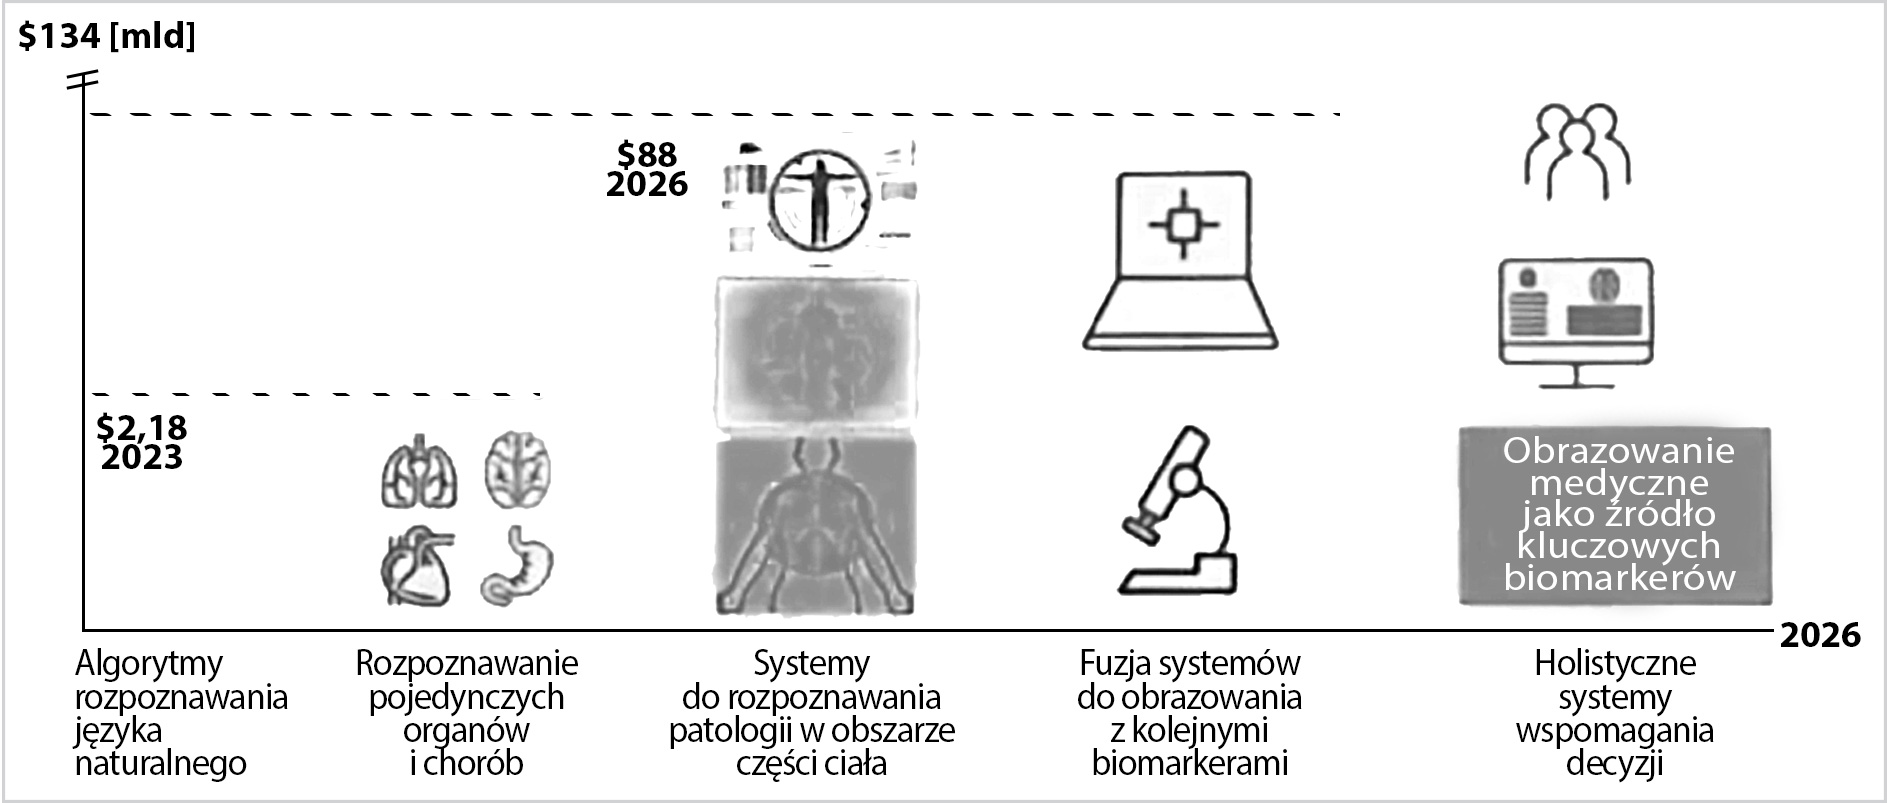
\includegraphics[width=\textwidth]{figures/Pred_AI.jpg}
	\caption{Przewidywania rozwoju możliwości systemów opartych o metody AI w radiologii według firmy IBM.}
	\label{fig:IBM_pred}
\end{figure}
Rozwój ma postępować od obecnych metod identyfikujących wybrane parametry przez systemy holistyczne rozpoznające patologie całych struktur anatomicznych i w konsekwencji wspomagające diagnostykę całego organizmu ludzkiego. Kolejnym etapem powinna być integracja z biomarkerami pochodzącymi z poza obszaru obrazowania medycznego, co w konsekwencji ma w pełni symulować pracę klinicysty i stać się systemem autonomicznym. W opinii autora tej pracy kwestią sporną jest data podana przez firmę IBM tj. 2026. Biorąc pod uwagę złożoność problemu (opisaną po części w tej pracy), kwestie legalne i etyczne, perspektywa czasowa wydaje się być trudna do osiągnięcia. Niemniej jednak proponowane, przedmiotowe rozwiązanie żywotnie wpisuje się w kolejne, przewidywane etapy. Obecnie proponowane podejście opisane w p. \ref{NewMethod} bazuje na wyliczeniu 6-ciu parametrów charakteryzujących sygnał RM widoczny w badaniu ścięgna Achillesa. Jeden z parametrów tj. TT dodatkowo niesie informacje geometryczne o pogrubieniu struktury. W celu oceny holistycznej (etap II) ścięgna konieczna jest finalizacja prac z zakresu segmentacji ścięgna i dołączenie pełnego opisu geometrycznego. Wówczas w naturalny sposób rozwiązanie mogłoby być zintegrowane do opisu całego organizmu ludzkiego (etap III). Omówione wcześniej testy funkcjonalne oraz organoleptyczne (np. palpacyjne), jak również np. próbki tkanek czy badania epigenetyczne stanowią bazę dodatkowych biomarkerów (przykłady podano w p. \ref{seq:comp-biomechanics}), które wymagają integracji w celu działań w pełni autonomicznych w zakresie oceny na etapach IV i finalnie V. Z wykorzystaniem badań zawartych w tej pracy autor ma nadzieję na dokończenie etapu I i realizację kolejnych etapów w ramach działań związanych ze spółką spin-off Uniwersytetu Warszawskiego. 

\chapter{Podsumowanie}

W ramach pracy osiągnięto wszystkie założone we wstępie cele. Cel główny tj. opracowanie automatycznej metody oceny gojenia się ścięgna Achillesa został osiągnięty poprzez zastosowanie unikatowej fuzji cech wyuczonych przez model głębokiej sieci neuronowej i cech wyekstrahowanych z wykorzystaniem klasycznych metod przetwarzania obrazów. Wnioski zostały spisane w Rozdziale \ref{NewMethod} podzielonym na trzy sekcje. W pierwszej przedstawiono szczegółowy opis komponentów oraz ich parametrów wraz z unikatowymi w skali światowej danymi (zob. p. \ref{seq:method}). W drugiej zaprezentowano wyniki eksperymentów mających na celu dobór komponentów i ich parametrów oraz optymalizację czasu, jakości i kosztów związanych z zastosowaniem nowej metody (zob. p. \ref{seq:experiments}). W ostatniej, trzeciej sekcji, zaprezentowano szczegółową walidację wraz z analizą rozbieżności między nowym podejściem, a oceną radiologa (zob. p. \ref{seq:valuation}).

W toku prac, zrealizowano również wszystkie cztery cele szczegółowe. Pierwszy, tj. "Wybór efektywnego kosztowo i czasowo protokołu badania bazującego \linebreak na technikach obrazowania medycznego, a dokładniej Rezonansu Magnetycznego" zrealizowano poprzez badania zamieszczone w p. \ref{seq:protocol_selection}. Najważniejszym rezultatem tych prac jest określenie utylitarnego protokołu badania składającego się tylko \linebreak z jednej, trwającej przy obecnym stanie techniki około 5 min. sekwencji RM. 

Drugi cel, tj. "Przetestowanie różnego rodzaju podejść związanych ze szkoleniem głębokich sieci neuronowych" zrealizowano poprzez zestawienie wyników działania nowej metody z wynikami alternatywnego podejścia tj. szkolenia sieci w oparciu \linebreak o paradygmat end-to-end (zob. p. \ref{seq:end-to-end}). W zestawieniu z alternatywną metodą analizy obrazów RM, wykazano przewagę zaproponowanego podejścia, a dokładniej uzyskano wyższe rezultaty korelacji w każdym z sześciu ocenianych parametrów oraz dla czterech z nich niższy absolutny błąd średni.

Kolejny cel, tj. "Porównanie wyników oceny nowej metody z wynikami klasyfikacji bazującej na danych z ultrasonografii" zrealizowano dołączając do pracy wyniki automatycznej interpretacji obrazów USG (zob. p. \ref{seq:comp-usg}). W szczególności wykazano możliwość synergii obu podejść, bazując na większej izotropowości danych USG \linebreak i dobrych wynikach oceny parametrów widocznych w płaszczyźnie strzałkowej.

Ostatni cel, tj. "Porównanie wyników oceny nowej metody z oceną funkcjonalną, rutynowo stosowana do wspomagania rehabilitacji po urazie ścięgna" osiągnięto uzyskując unikatowe dane pomiarów biomechanicznych i testu ATRS, a następnie zestawiając je z wynikami nowo-opracowanej metody (zob. p. \ref{seq:comp-biomechanics}). Pokazano przydatność wykonywania badań radiologicznych, przez wzgląd na odmienność niesionej informacji. Jednocześnie określono potencjalny obszar optymalizacji w zakresie istotnej statystycznie korelacji proponowanej oceny automatycznej z wynikami testu ATRS.  

W ramach powyższych prac nad nowym podejściem do oceny procesu gojenia się ścięgna Achillesa w badaniach RM, całość zadań dotyczących głębokich sieci neuronowych została zrealizowana przez autora tej pracy. Pełnił on również rolę głównego badacza, projektując i współrealizując prace nad fuzją cech (w szczególności w ramach testów perceptronu wielowarstwowego i SVR jako typów meta-regresji). Autor tej pracy nadzorował również i planował eksperymenty grupy tworzącej metody bazujące na paradygmacie end-to-end oraz wykorzystywane do interpretacji obrazów USG. Następnie samodzielnie dokonał ich porównania z proponowanym w tej pracy podejściem. 

Wszystkie wyniki mają charakter innowacyjny. Nie istnieje obecnie, wedle najlepszej wiedzy autora tej pracy, alternatywne podejście do usystematyzowanej i wyliczanej automatycznie oceny stanu gojenia się ścięgna Achillesa widocznego w badaniach RM. Rozprawa ta stanowi zatem kompleksowy opis obecnego \textit{state-of-the-art} dla przedmiotowego problemu. Biorąc pod uwagę, że w przedstawionym stanie najlepsze wyniki oceny automatycznej korelują z oceną radiologa na poziomie 0,85, a minimalny uzyskany absolutny błąd średni równy jest 0,56, krytyczne w opinii autora tej pracy staje się polepszenie wzorca odniesienia. 

Planowana jest zatem dalsza, stała współpraca z radiologami i decydentami celem realizacji ocen przez kolejnych specjalistów oraz wieloośrodkowe zbieranie nowych wolumenów danych. Przewidziane jest także przeprowadzenie badań w zakresie usprawnienia przetwarzania danych, w szczególności w kwestii automatycznej segmentacji ROI. Zrealizowane prace stanowią również fundament pod rozpoczęcie nowych testów, dotyczących pokrewnych zadań, jak ocena gojenia się podobnych struktur np.: więzadeł stawu kolanowego, skokowego, barkowego, czy łokciowego. 

Polepszenie skuteczności wspomagania rehabilitacji w obszarze układu mięśniowo-szkieletowego stanowi według autora tej pracy ciekawe wyzwanie badawcze, jak również ma wymiar praktyczny. Już teraz bowiem, według danych Krajowej Izby Fizjoterapeutów, po zwolnieniach z pracy dotyczących ciąży, zwolnienia na skutek dolegliwości mięśniowo-szkieletowych stanowią drugi powód absencji w pracy w Polsce. \linebreak W odpowiedzi na rosnący problem, w ramach otrzymanego przez autora tej pracy i mgr. Bartosza Boruckiego w Czerwcu 2019 roku grantu z programu Inkubator Innowacyjności 2.0, organizowanego przez ministra nauki i szkolnictwa wyższego, planowana jest realizacja wyżej wymienionych prac i przygotowanie do wdrożenia przedmiotowego rozwiązania. Działania pozwolą na usprawnienie rehabilitacji ścięgna Achillesa oraz jego profilaktyki, jak i rozpoczęcie badań nad opracowaniem rozwiązań dedykowanych do wspomagania leczenia innych, podobnych urazów.


%- jeden radiolog więc ankieta ok
%- AlexNet uczy się bardziej generycznych cech niż ResNet, który zwraca uwagę na szczególy: https://www.researchgate.net/post/Can_AlexNet_be_a_better_feature_extractor_than_ResNet

%https://icmlviz.github.io/icmlviz2016/assets/papers/4.pdf

%Wydzielenie stanu przed operacją i oznaczenie osobną etykietą w procesie treningu mogłoby doprowadzić do polepszenia rezultatu, co jest sugestią dla przyszłych prac związanych z rozwojem metody.

%TU - Polepszenie w zakresie oceny tego parametru może być uzyskane w przypadku zastosowania bardziej jednorodnych danych RM lub USG.

